\SubSection{Analysis: Course Project - Test vs. Total Code}

\begin{figure}[ht]
  \centering
  \includegraphics[width=0.5\textwidth]{course-project-analysis-loc-2.eps}
  \caption{Course Project - Test vs. Total Code}
  \label{fig:course-project-analysis-loc}
\end{figure}


For example, Figure \ref{fig:course-project-analysis-loc} provides a
comparative view of the size of each of the systems (including both test
code LOC and total LOC) over a given time interval.  Course analyses are
designed to identify only the data associated with the given user's project
(in this case ``Sitewatch-Ewalu''); other projects are left unidentified. 
The example analysis shows several positive things about the
Sitewatch-Ewalu project during this interval: there were changes made to
the code by some team member each day (indicating consistent
effort). In contrast, some of the other teams had a ``N/A'' listing for one
or more days, indicating no changes to the code.  The size of code
developed is appropriate relative to other projects, as is the percentage
of code devoted to testing. 

